%% Autor: Björn Ritterbecks 
%% Letzte Aenderung: 15.06.2016 
\thisfloatsetup{%
  capbesidewidth=\marginparwidth,
    capbesideposition=top,
    postcode=flushupp}
\begin{figure*}[htbp]
\centering
%\sansmath
 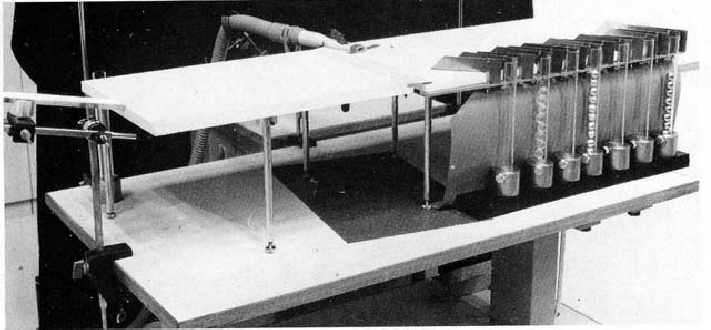
\includegraphics[width=0.99\fulllinewidth]{images/mnu.png}
  \caption[Analogieversuch zu Massenspektrometrie nach \textsc{Luchner}, \textsc{Degner} und \textsc{Schilling} ]{\protect\rule{0cm}{7.6cm}Mechanisches Funktionsmodell eines geschwindigkeitsfokussierenden Massenspektrographen nach \textsc{Schilling} et al.: Kugeln unterscheidbarer Dichte werden die v-förmige Rampe an der linken Seite heruntergerollt, wo sie auf einer schiefen Ebene nach ihrer Geschwindigkeit sortiert werden. Auf der rechten Seite sorgt das Strömungsfeld eines Gebläses für eine Aufspaltung nach den Impulsen (entnommen aus \cite[S\,35]{Schilling1987}).}
  \label{fig:mnu}
  \vspace{-0pt}
\end{figure*}